\documentclass{beamer}

\usepackage{xfrac}

\usetheme{default}

\title{NBICS Technologies}
\author{Alexander Aksentyev}
\institute{National Research Institute ``MEPhI''}
\date{}


\begin{document}
	\begin{frame}
		\titlepage
	\end{frame}

\section{Nano-technologies}

\begin{frame}
	\frametitle{Carbon allotropes}
	\begin{columns}
		\column{.4\textwidth}
		Allotropy is the property of some chemical elements to exist in several different geometries (known as \emph{allotropes}) in the same physical phase.
		\column{.6\textwidth}
		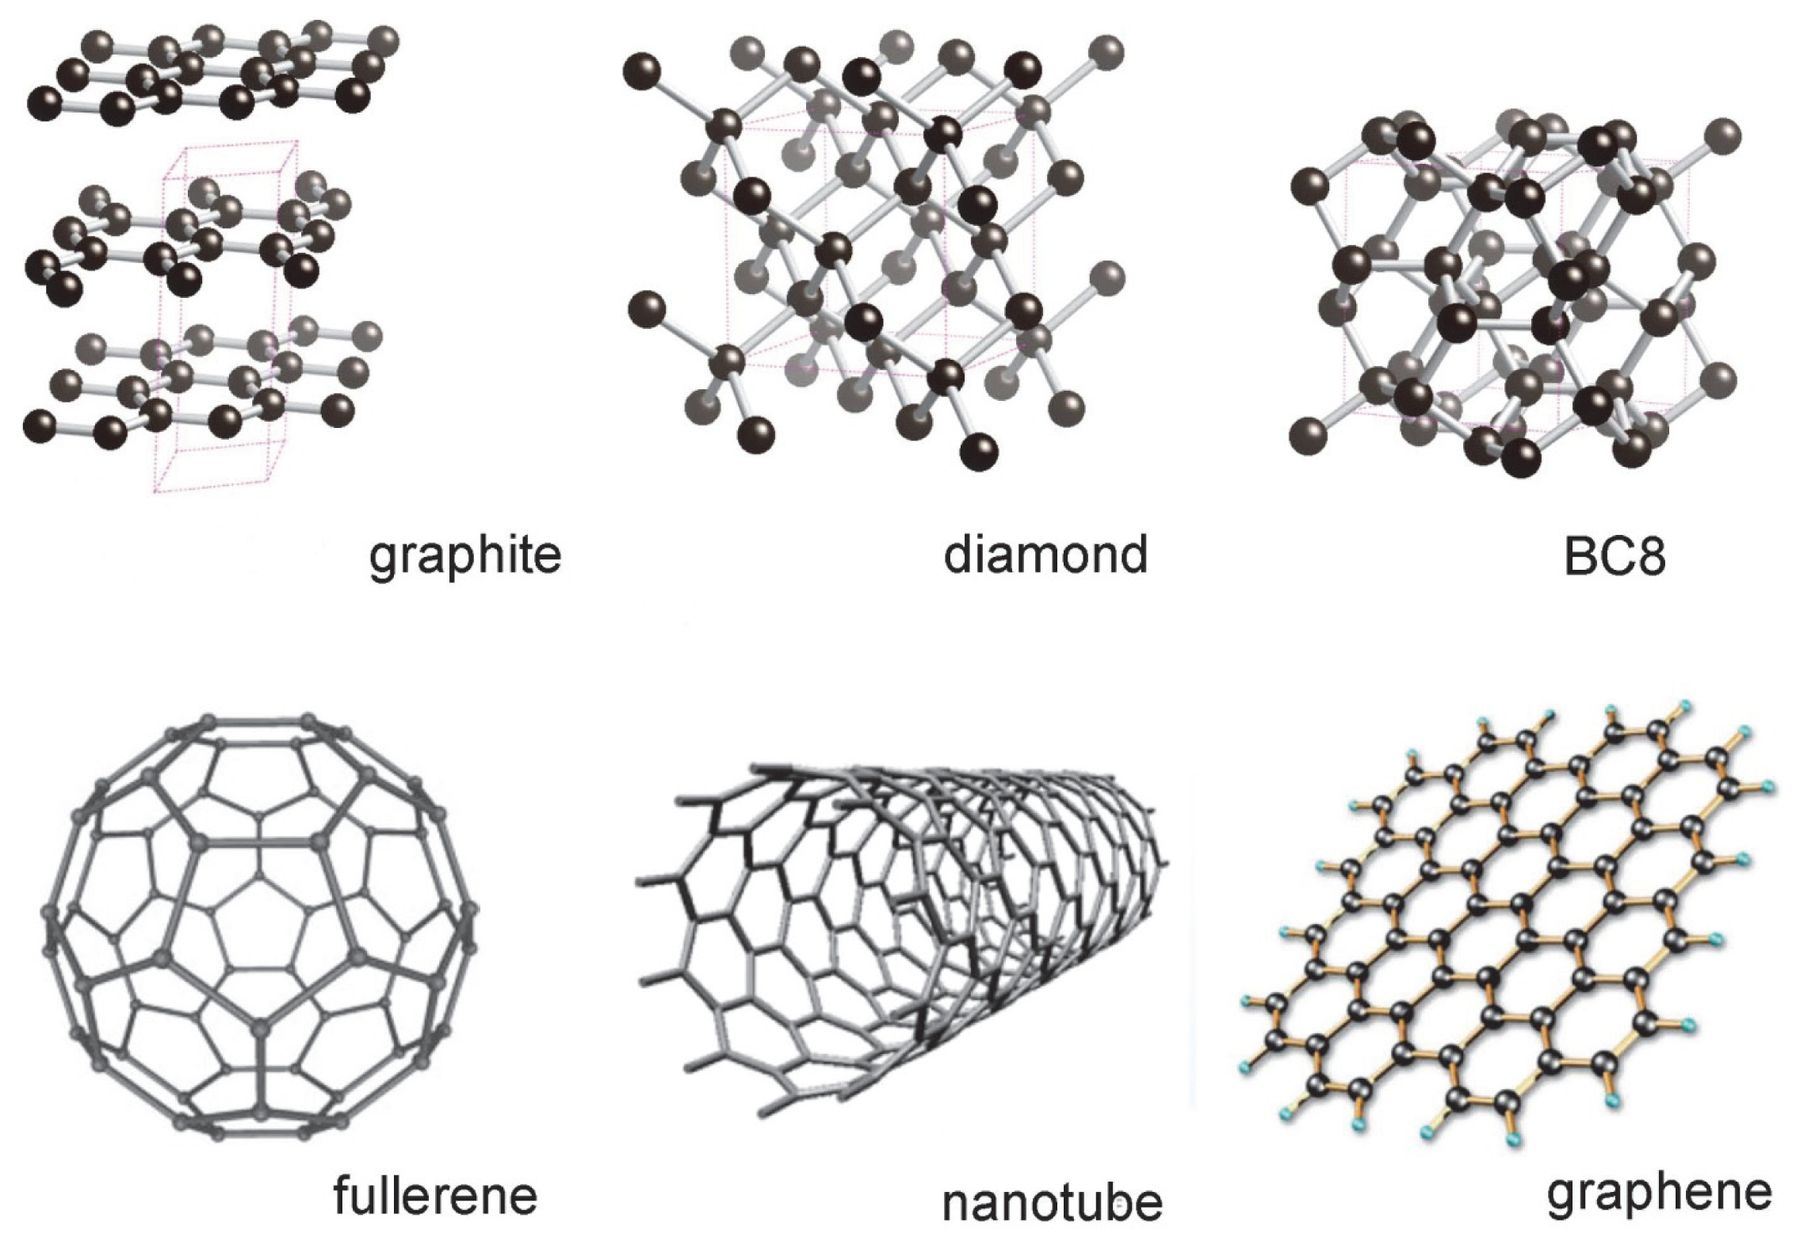
\includegraphics[scale=.45]{CarbAllotropes}
	\end{columns}
\end{frame}

\begin{frame}
	\frametitle{The Buckyball}
	\begin{columns}
		\column{.7\textwidth}
		\begin{itemize}
			\item The Buckminsterfullerene (named after inventor Richard Buckminster Fuller) was one of the first nanoparticles to be discovered (1985)
			
			\item Number of atoms: 20 to over 100; the most common type (C60) contains 60 carbon atoms
					
			\item Modifying a buckyball by adding or replacing an atom in order to change the properties of the buckyball is called \textbf{functionalization}
		\end{itemize}
		\column{.5\textwidth}
		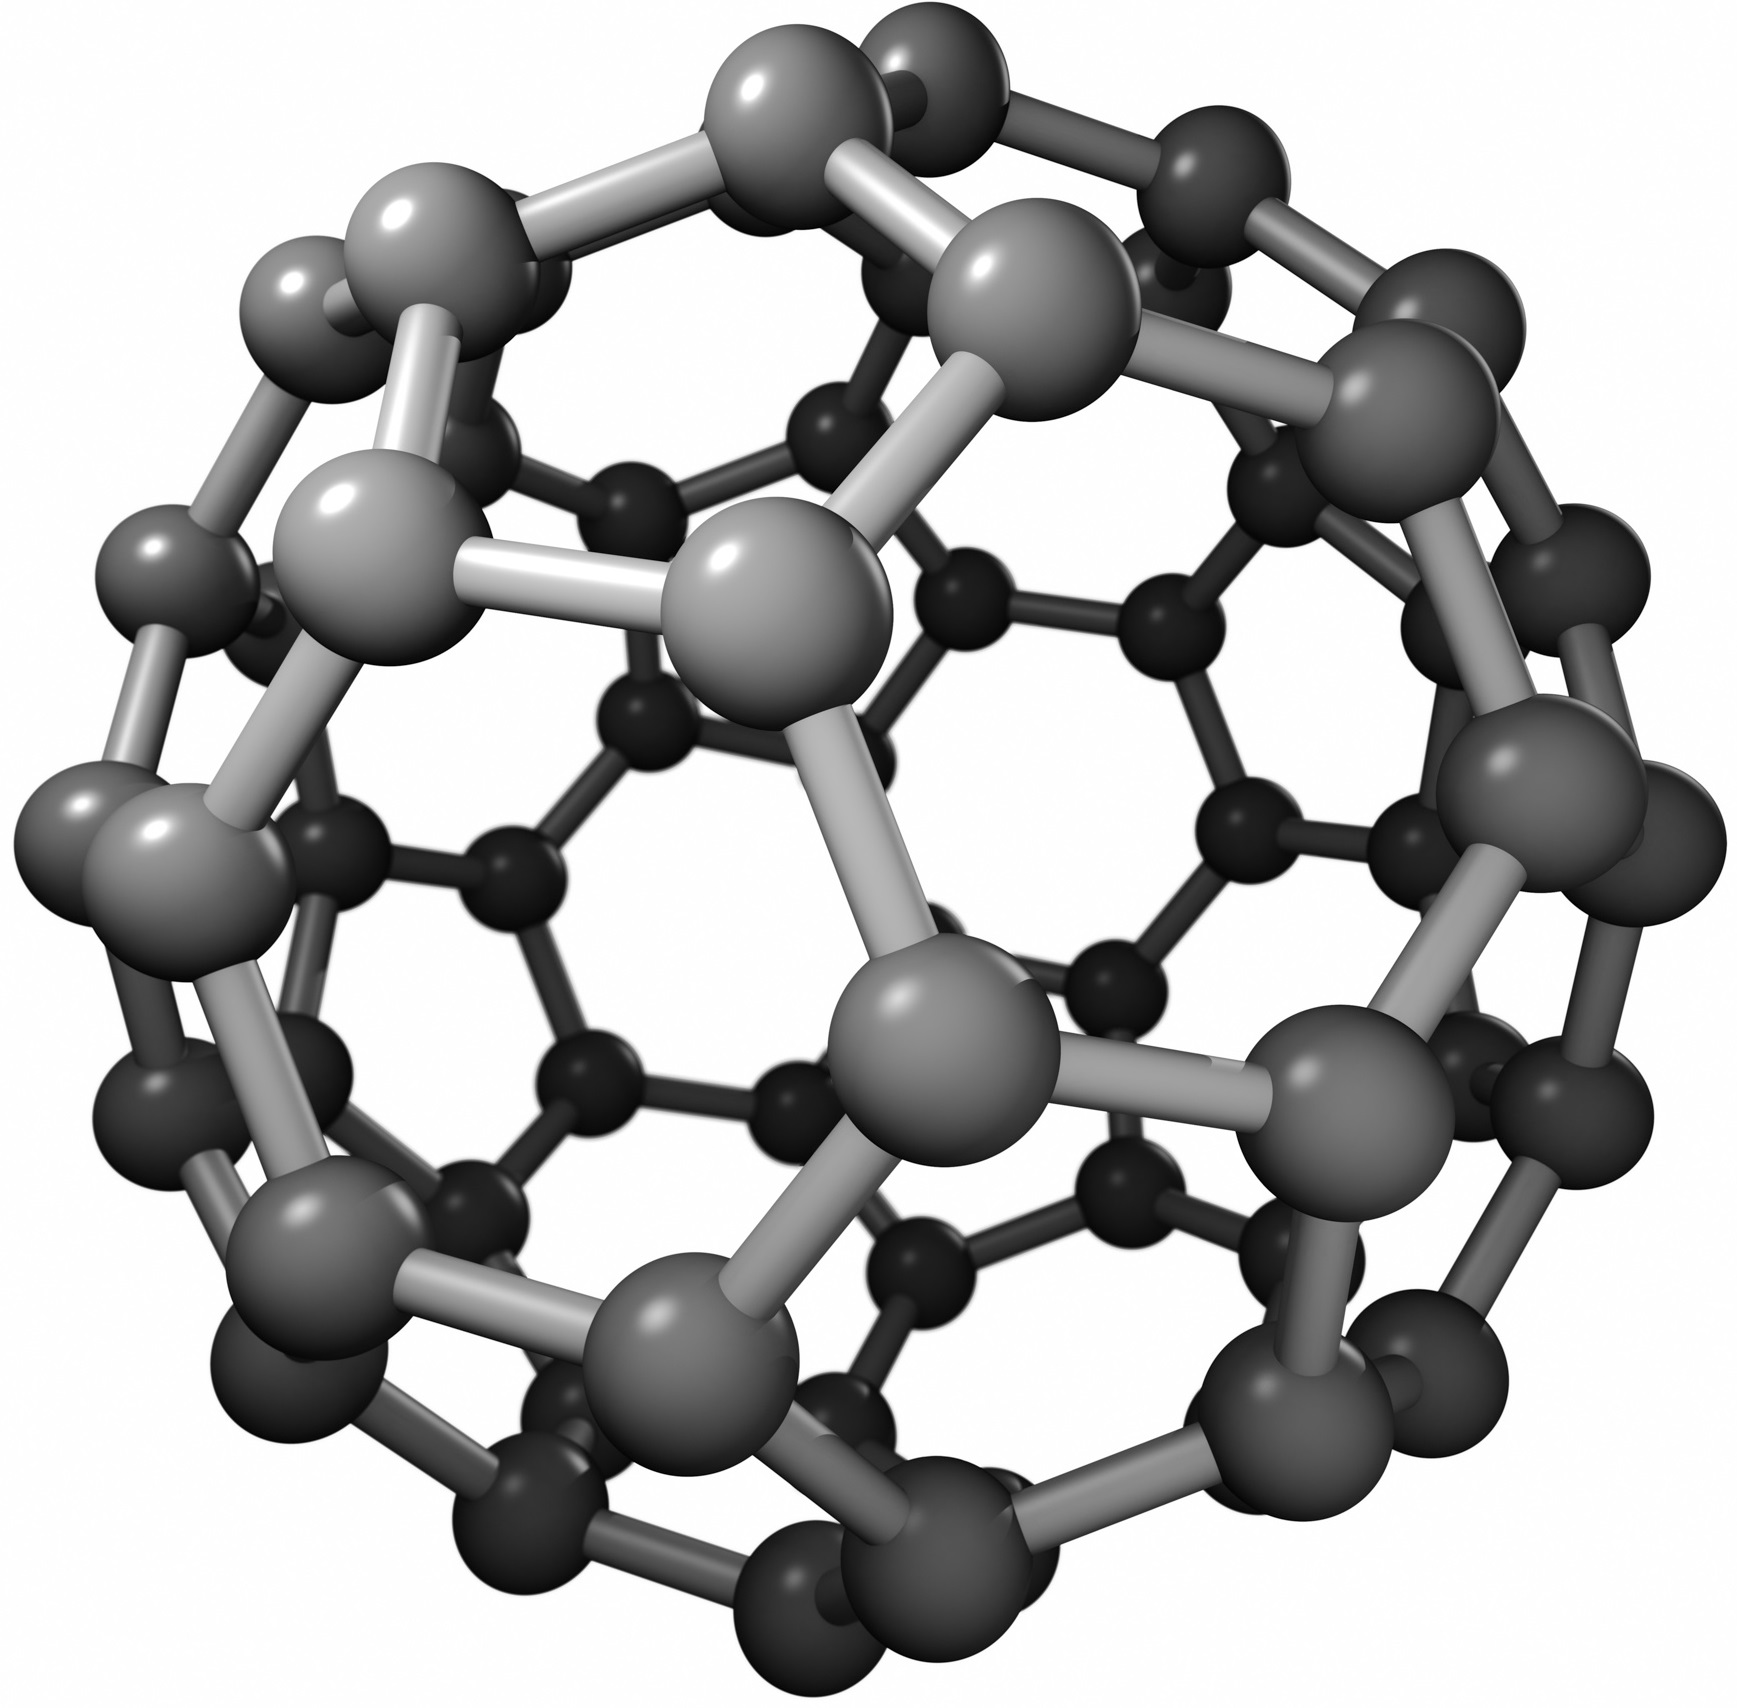
\includegraphics[scale=.2]{buckyball_white}
	\end{columns}
\end{frame}

\begin{frame}
	\frametitle{Uses}
	\begin{itemize}
		\item \textbf{Armor}. Hard as diamonds, buckyballs are potentially useful within armor
		
		\item \textbf{Medicine}. Functionalized buckyballs can be made soluble by body cells, and hence find the following medical applications:
			\begin{itemize}
				\item As antioxidants, because of their ability to absorb electrons in free radicals
				
				\item In targeted drug delivery. The buckyball encases a minute dose of a particular drug. By controlling the functionalization of the buckyball the drug remains encased until the buckyball reaches the site where the drug is required. The buckyball then releases it
			\end{itemize}
		\item \textbf{Fiber optics}. Because of their perfect spherical shape, bucky balls are able to transmit light

	\end{itemize}
\end{frame}

\begin{frame}
	\frametitle{The nanotube}
	\begin{columns}
		\column{.5\textwidth}
		\begin{itemize}
			\item Diameter $<$ 1 nm
			\item A few nano- up to a millimeter in length
			\item Symmetry: armchair, zig-zag, chiral
			\item Single/multiple wall CNTs
			\item Compared to steel:
				\begin{itemize}
					\item 100 $\times$ more difficult to tear apart
					\item 5 $\times$ as elastic
					\item a quarter density
				\end{itemize}
			\item High thermal conductivity
			\item Metallic/semi-conductive contingent on symmetry
		\end{itemize}
		\column{.65\textwidth}
		\begin{minipage}{.5\textheight}
			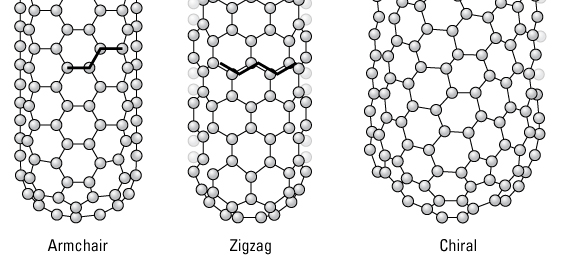
\includegraphics[scale=.65]{nanotube_orientations}
		\end{minipage}
	\begin{minipage}{.5\textheight}
		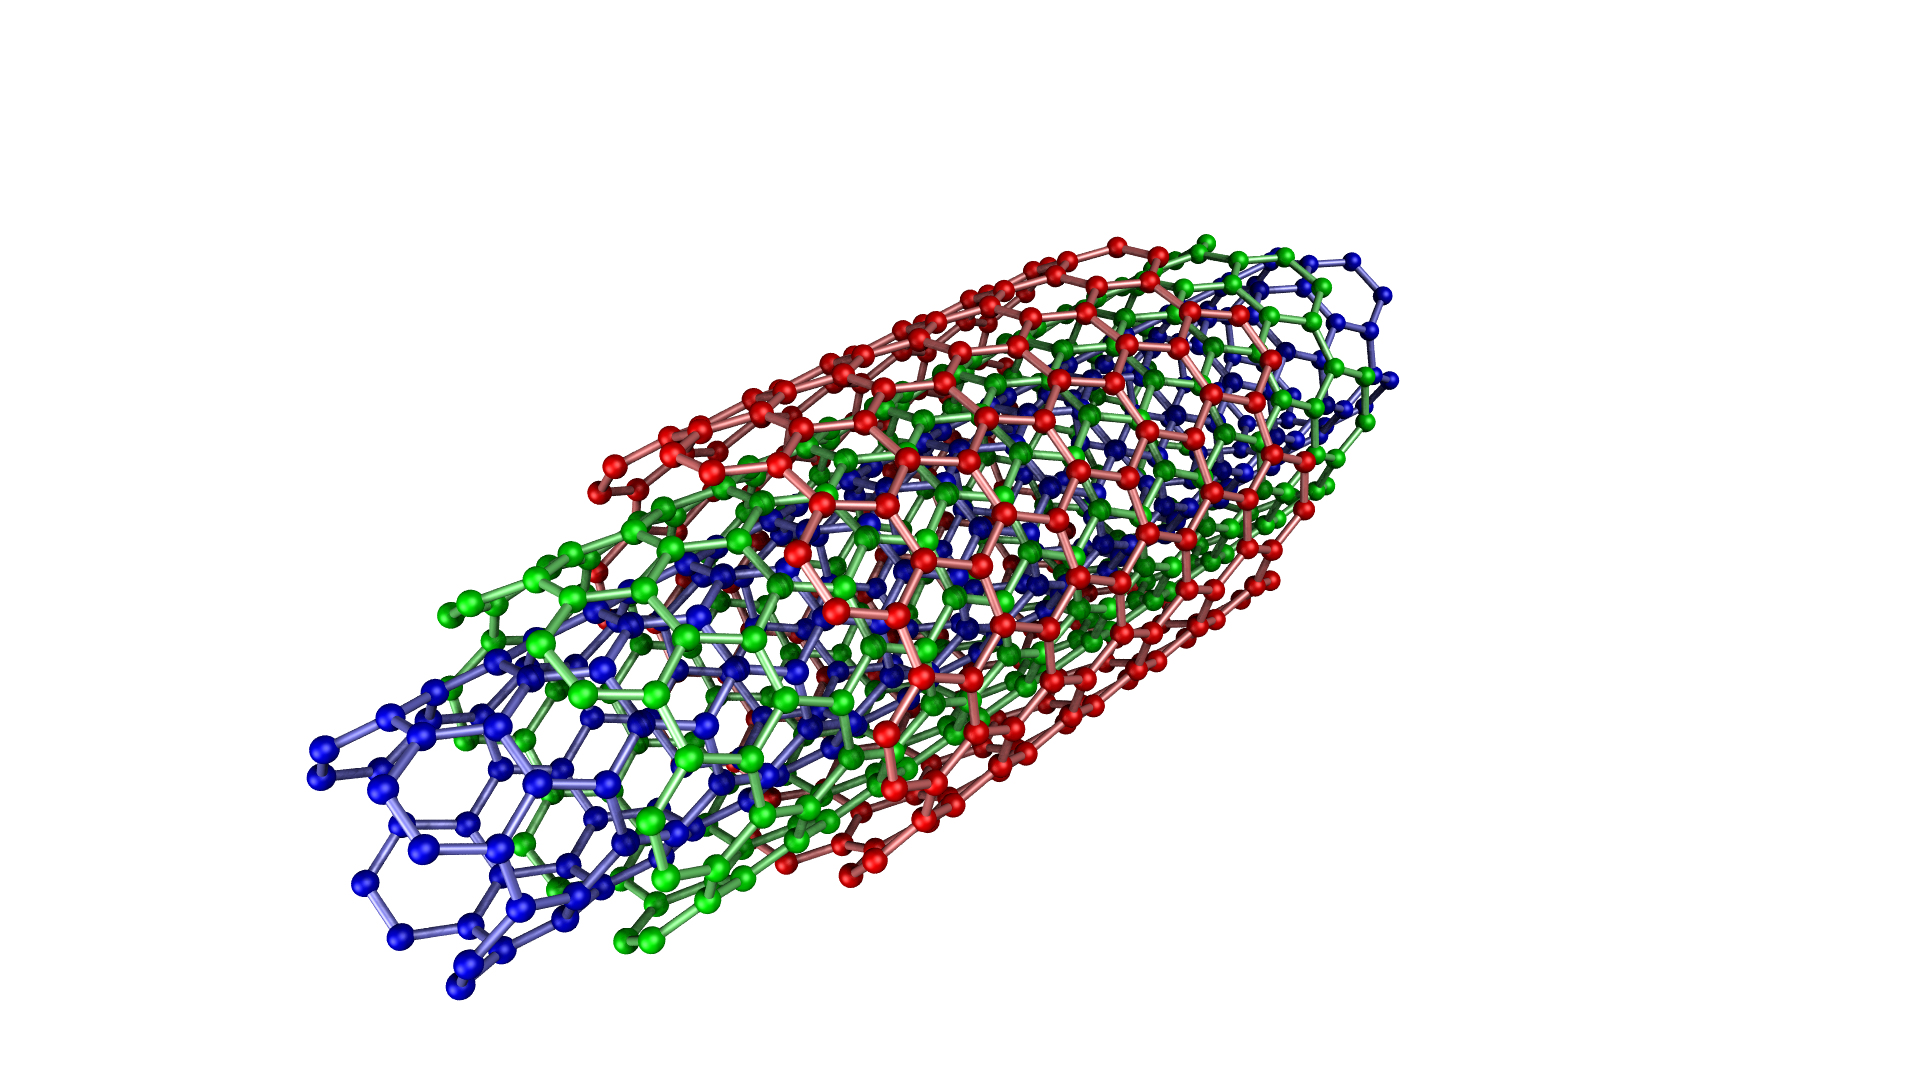
\includegraphics[scale=.1]{MWCNT}
	\end{minipage}
	\end{columns}
\end{frame}

\begin{frame}
	\frametitle{Uses}
	\begin{enumerate}
	\item \textbf{Medicine}: functionalization, as well as their natural fluorescence, enable the use of CNTs as chemical sensors; they have also been shown to fuse well with bone, which could be used to diminish the implant rejection rate
	\item \textbf{Conductive plastics}: CNTs are the best known conductive fillers because of their high aspect ratio
	\item \textbf{Energy storage}: good battery electrodes due to high surface area ($\sim 1000$ m$^2$/g), good electrical conductivity, and linear geometry; the high surface area and thermal conductivity also make them useful as electrode catalysts in fuel cells
	\item \textbf{Molecular electronics}: their geometry, electrical conductivity, and the ability to be precisely derived, make CNTs invaluable connectors between switches at the nanoscale; their properties as semiconductors also make them usable as switches themselves
	\end{enumerate}
\end{frame}

\begin{frame}
	\frametitle{The nanobud}
	\begin{columns}
		\column{.5\textwidth}
			A nanobud is a nanotube with a fullerene ball attached to it.
		\column{.5\textwidth}
			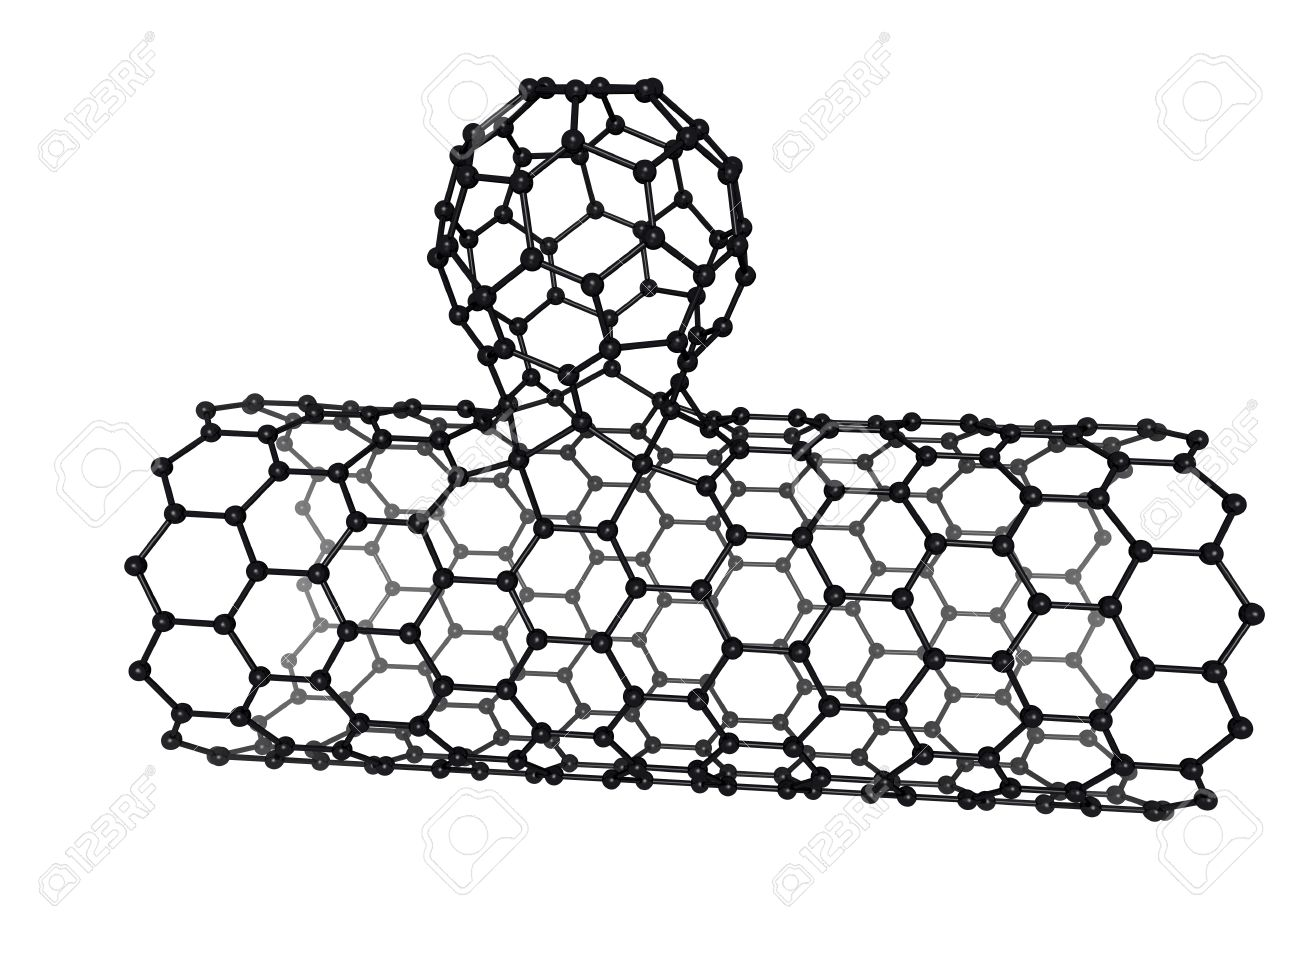
\includegraphics[scale=.15]{Nanobud}
	\end{columns}
\end{frame}

\section{Bio-technologies}

\section{Info-technologies}

\section{Cogno-technologies}

\section{Socio-technologies}

\end{document}